\exercise{Control}
In robotic locomotion it is common to abstract from the robot by using inverted pendulum models.
In this exercise we will use a planar double inverted pendulum to test different control strategies. Our robot can be controlled by specifying the torque $\mathbf{u}=[u_1, u_2]$ of its motors. Consider that in mechanical systems the torque $\vec{u}$ is a function of the joint positions $\vec{q}$, velocities $\dot{\vec{q}}$ and accelerations $\ddot{\vec{q}}$, as given by  
\[
\vec{u}=\vec{M}(\vec{q})\ddot{\vec{q}}+\vec{c}(\vec{q},\dot{\vec{q}})+\vec{g}(\vec{q}), 
\] 
where $\vec{M}$ denotes the inertial matrix, $\vec{c}(\vec{q},\dot{\vec{q}})$ the Coriolis and centripetal forces, and $\vec{g}$ the gravity terms. In the following exercises assume that these terms are given.

For the programming exercises you will use the attached code. 
We provide skeletons for controlling the system either in joint space (\texttt{my\_ctl.py}) or in task space (\texttt{my\_taskSpace\_ctl.py}) and a basic functionality for plotting. You can invoke either mode by running \texttt{jointCtlComp.py} or \texttt{taskCtlComp.py} respectively. 
Attach a printout with plots and a snippet of your source code for each programming exercise. 

\begin{questions}
	
	%----------------------------------------------
	
	\begin{question}{PID Controller}{2}
		What is the form of a proportional-integral-derivative (PID) controller and how could you use it to control a robot, i.e. what physical quantities could you control? Name one positive and one negative aspect of PID controllers.
		
\begin{answer}
	     Form of a PID controller: $u(t)=K_P e(t)+K_I \int_{- \infty}^{t} e(\tau)d\tau +K_D \frac{de(t)}{dt}, \qquad e(t) = q_{desired}-q$
	     
	     Quantities to control: \\
	     \begin{tabular}{l l}
	     	KP & Proportional part adjusts the gain of the control loop. Increasing the gain makes it faster. \\
	     	KI & Integral part used to prevent any residual steady state error.\\ &Caution if the KI is to high overshooting the set point is likely \\
	     	KD & Derivative part improves the settling time and the stability of the system.\\& (Caution: an ideal derivative is not causal)\\
	     \end{tabular}
	     
	     Compared to PD,P Controllers, PID Controllers have no steady state error. However if the model is not precisely known it is not advisable to use PID controllers especially not for tracking control. Moreover you should keep in mind, that a WINDUP might occur. 
	     
	\end{answer}
		
	\end{question}
	
	%----------------------------------------------
		
	\begin{question}{Gravity Compensation and Inverse Dynamics Control}{4}
		Suppose that you would like to create a control law to set the joint angles on the double inverted pendulum model by controlling the torque of the motors. Write a feedback control law which additionally gravity compensates and then extend it to full inverse dynamics control. 
		
\begin{answer}
				\begin{center}
					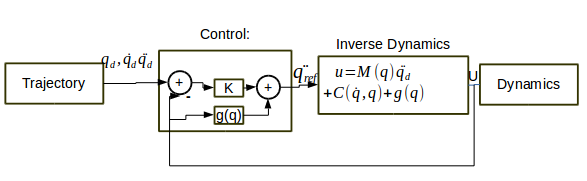
\includegraphics[width=0.7\textwidth]{img/2b.png} 
				\end{center}
				
				$\ddot{{q}}_{ref}={\ddot{q}}_d+K_D(\dot{q}_{des}-\dot{q})+K_P(q_{des}-q)+g(q)$
	\end{answer}
		
	\end{question}
	
	%----------------------------------------------
	
	\begin{question}{Comparison of Different Control Strategies}{12}
		In the following exercise you will investigate the differences of the following control algorithms, P, PID, PD with gravity compensation, and full inverse dynamics.
		The double pendulum is initiated hanging down, with state $\vec{q_\textrm{start}}={[-\pi,0]}$. We simulate the system with a time-step $dt=0.002$ seconds using symplectic Euler integration and run the simulation for $t_\textrm{end}=3s$. 
		
		Implement the control laws by filling the skeleton file \texttt{my\_ctl.py}. Use the following feedback gains $K_P=60, K_D=10, K_I=0.1$ for the first joint and $K_P=30, K_D=6, K_I=0.1$ for the second one.
		The target state of the double pendulum is set to $\vec{q_\textrm{des}}={[-\pi / 2,0]}$. 
		
		Create (max. 4) plots that compare the different control strategies and analyze the results. It is your choice how to illustrate your results. In your analysis you should include a discussion on the overall performance of each controller. Which controllers manage to go to the desired point, and how does the choice of a controller affects the behavior of the second joint of the pendulum? Additionally discuss which controller you would choose and why. The provided code is able to generate plot but feel free to modify it if you like. Points will be deducted for confusing plots. Do not forget to include your source code in your solutions.
		
\begin{answer}
\begin{minipage}{0.7\textwidth}
	\begin{figure}[H]
		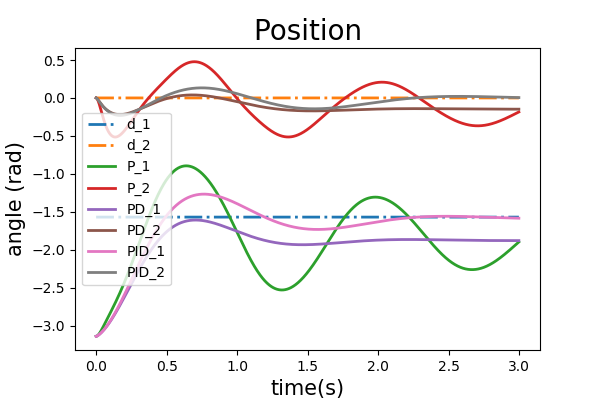
\includegraphics[width=1\textwidth]{img/2cpos1.png} 
		\caption{\label{fig:2cpos1} Comparing the position of the P,PD,PID controller}
	\end{figure}
\end{minipage} \hfill
\begin{minipage}{0.25\textwidth}
	First of all we compare the positioning behavior of the P,PD and PID controller. In figure \label{fig:2cpos1} we can see, that the P controller oscillates around the desired position. The PD controller has a steady state error. Only the PID controller behaves nicely and has no steady state error and does not overshoot the set point too much. Moreover the PID controller is not oscillating.
\end{minipage}

\begin{minipage}{0.7\textwidth}
	\begin{figure}[H]
		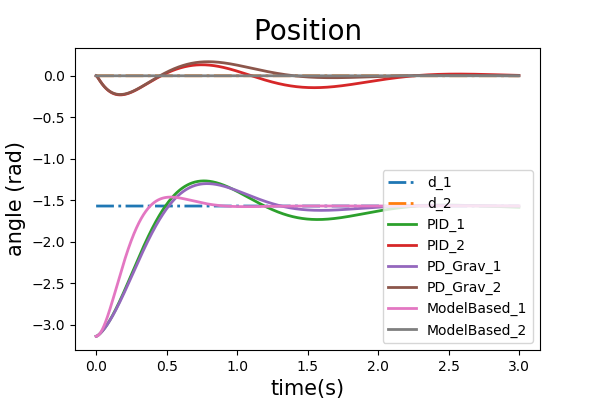
\includegraphics[width=1\textwidth]{img/2cpos2.png} 
		\caption{\label{fig:2cpos2} Comparison of the position of PID, PD\_GRAV and MPC}
	\end{figure}
\end{minipage} \hfill
\begin{minipage}{0.25\textwidth}
	The PD\_Grav. controller reaches the desired position of joint2 faster than the PID controller. However this costs a little bit more overshooting. Comparing all 3 controllers in figure \ref{fig:2cpos2} it is clear that the model based controller has the optimal positioning behavior. For joint1 it reaches the desired position quickest with minimal overshooting. In case of joint2 the model based controller is able to not oscillate at all.
\end{minipage}

\noindent\begin{minipage}{.5\textwidth}
	\centering
	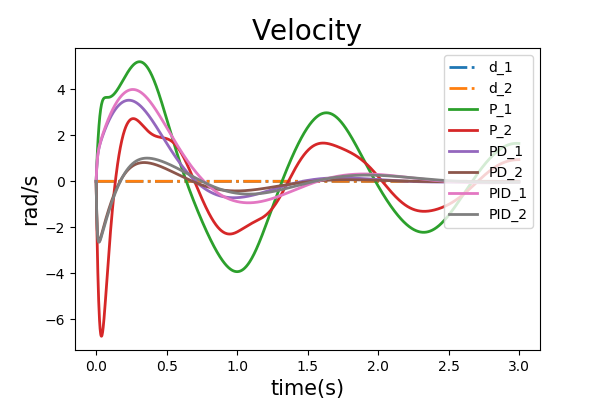
\includegraphics[width=1\textwidth]{img/2cvel1.png} 
	\captionof{figure}{Comparing the velocity of the P,PD,PID controller}
	\label{fig:2cvel1}            
\end{minipage}%
\begin{minipage}{.5\textwidth}
	\centering
	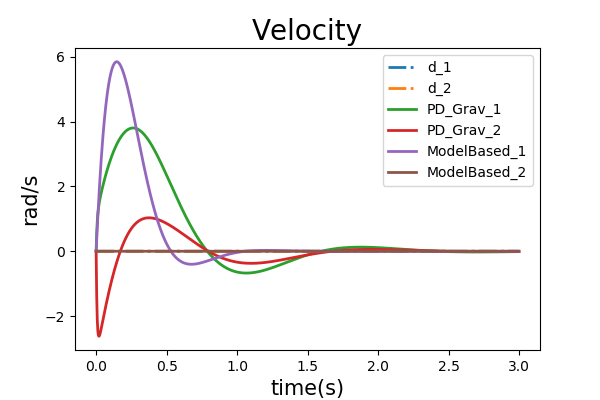
\includegraphics[width=1\textwidth]{img/2cvel2.png} 
	\captionof{figure}{Comparison of the velocity of PD\_GRAV and Model Based controller}
	\label{fig:2cvel2}               
\end{minipage}

Having a closer look to the velocity behavior of the controllers reveals that the all controllers (exept the P) reach the desired velocity of 0 rad/sec within 3 seconds. However again the model based controller is the fastest. 

In total it can be said the model based controller has the fastest positioning and velocity behavior of all controllers. Moreover it is the only one which is able to just stay at the desired position if the current position is equal to the desired position (see position for joint2). Neglecting any actuator saturation ("Stellgr\"ossenbeschr\"ankung") the model based controller is the best one. However if you have to care about an actor saturation you will probably not choose the model based controller, as it has the highest 
requirements on the actuators (see e.g. the high overshooting of the velocity (purpel line)). So if you have to care about actuator saturation the PD\_Grav is definitely better than the model based controller.

My\_clt.py:\\
\pythonexternal{src/myctl.py}

	\end{answer}

		
	
	\end{question}
	
	%----------------------------------------------
	
	\begin{question}{Tracking Trajectories}{4}
		Repeat the same experiment but this time use the provided time-varying target trajectory. Create (max 4) plots that compare the different control strategies and analyze the results. In your analysis discuss the overall performance and which controllers track the desired trajectory nicely. Additionally discuss which controller you would choose and why.
		
\begin{answer}
			\begin{minipage}{0.7\textwidth}
				\begin{figure}[H]
					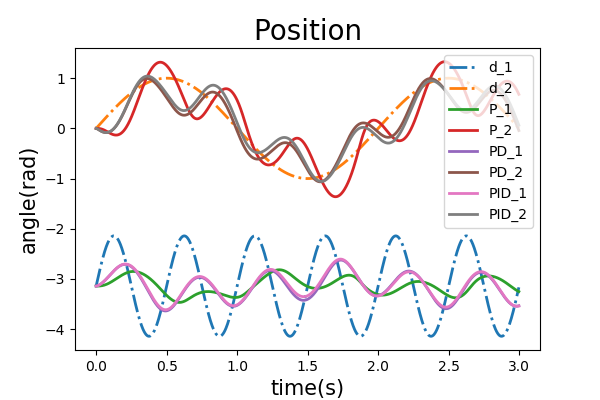
\includegraphics[width=1\textwidth]{img/2dpos1.png} 
					\caption{\label{fig:2dpos1} Comparison of the P,PD and PID positioning tracking behavior}
				\end{figure}
			\end{minipage} \hfill
			\begin{minipage}{0.25\textwidth}
				In figure \ref{fig:2dpos1} you can see that the tracking behavior of the P,PD,PID controllers fails. The desired positions of joint1 cannot be reached. Especially for joint1 we also can see that there is a time offset between the desired trajectory and the actual trajectories of the controllers.
			\end{minipage}
	
				\begin{minipage}{0.7\textwidth}
					\begin{figure}[H]
						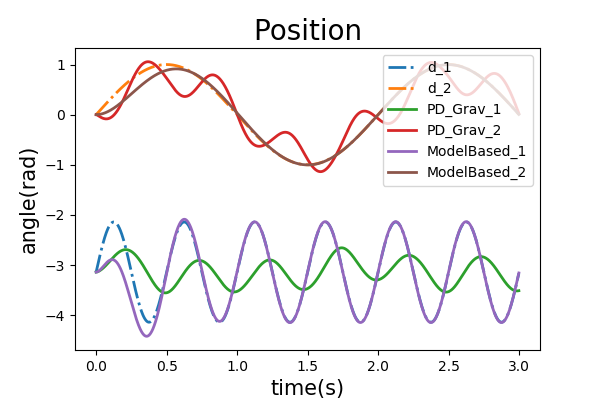
\includegraphics[width=1\textwidth]{img/2dpos2.png} 
						\caption{\label{fig:2dpos2} Comparison of the PD\_Grav. and model based controller's positioning tracking behavior}
					\end{figure}
				\end{minipage} \hfill
				\begin{minipage}{0.25\textwidth}
					In figure \ref{fig:2dpos2} you can see that the tracking behavior of the PD\_Grav and model based controllers differs a lot. The desired positions of joint1 and joint2 can only be reached by the model based controller. The PD\_Grav controller is faster than the P,PD,PID controller, however not fast enough to track the desired position of joint1 and joint2. It has a time offset and also does not reach the desired positions (see especially for joint1 green line).
				\end{minipage}
				
				\noindent\begin{minipage}{.5\textwidth}
					\centering
						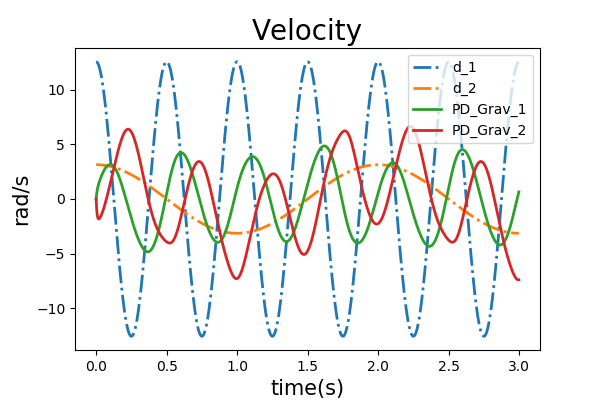
\includegraphics[width=1\textwidth]{img/2dvel1.png} 
					\captionof{figure}{The PD\_Grav tracking velocity behavior}
					\label{fig:2dvel1}            
				\end{minipage}%
				\begin{minipage}{.5\textwidth}
					\centering
					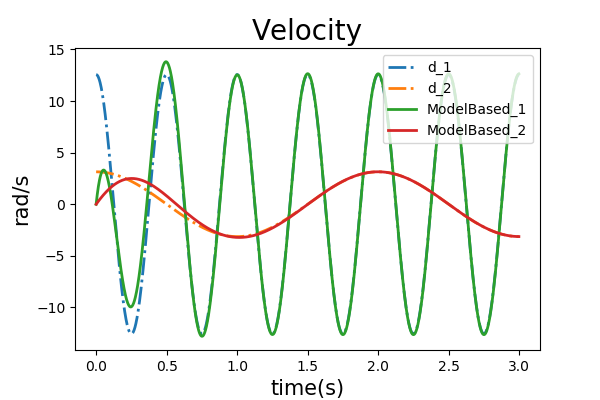
\includegraphics[width=1\textwidth]{img/2dvel2.png} 
					\captionof{figure}{The model based controller's velocity tracking behavior}
					\label{fig:2dvel2}               
				\end{minipage}
				
				Having a look at the two best positioning tracking controller's (the PD\_Grav and the model based) reveals, that their velocity tracking behavior also differs a lot. In \ref{fig:2dvel2} you can see that the velocity tracking behavior of the model based controller works perfectly well (with zero offset after some time), whereas the velocity behavior of the PD\_Grav controller fails (see \ref{fig:2dvel1}). In terms of tracking a trajectory the model based controller must be chosen, cause it is the only controller of the compared ones which is able to track a trajectory with zero offset. To track a trajectory a controller is required to reach a desired point fast enough with zero offset. This requirement is especially met by the model based controller.
	\end{answer}
		
	\end{question}
	
	%----------------------------------------------
	
	\begin{question}{Tracking Trajectories --- High Gains}{4}
		Repeat the same experiment (using the provided trajectory) but this time multiply the gains by ten. Create plots that compare the different control strategies and analyze the results. In your analysis discuss the overall performance and compare it to the previous case. Are there any drawbacks of using high gains?
		
\begin{answer}
	$K_{P,new}=K_{P,old}*10=[600,300]^T$ \\
	$K_{I,new}=K_{I,old}*10=[1,1]^T$\\
	$K_{D,new}=K_{D,old}*10=[100,60]^T$
	
					\noindent\begin{minipage}{.5\textwidth}
						\centering
						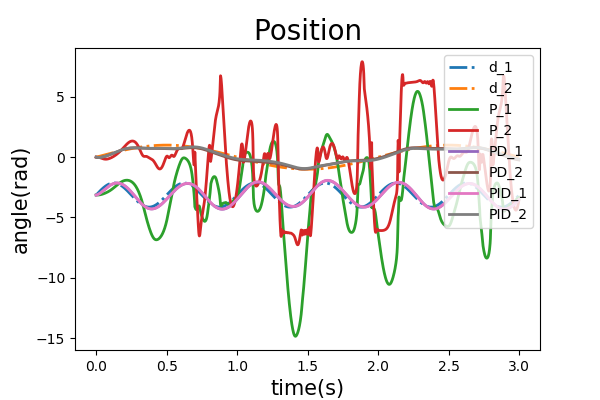
\includegraphics[width=1\textwidth]{img/2epos1.png} 
						\captionof{figure}{P,PD,PID position tracking behavior with high gains}
						\label{fig:2epos1}            
					\end{minipage}%
					\begin{minipage}{.5\textwidth}
						\centering
						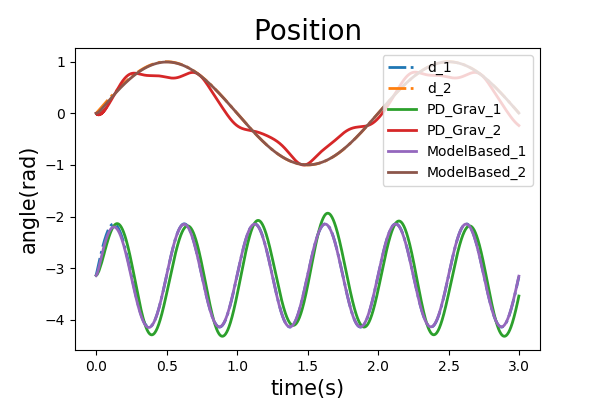
\includegraphics[width=1\textwidth]{img/2epos2.png} 
						\captionof{figure}{PD\_Grav, Model based position tracking behavior with high gains}
						\label{fig:2epos2}               
					\end{minipage}
	Having a look at figure \ref{fig:2epos1} one can see, that higher gains improve the positioning tracking behavior of the PD and PID controller. However the P controller's tracking behavior is worse (compared to d) ) cause it shows unstable behavior. So it can be concluded that higher gains might destabilize a system. The PD and PID controller however work better(compared to d) ), because increasing their gains results in a faster step response and now both controllers are fast enough to track the desired trajectory. Due to the derivative part these two controllers are also stable. Having a close look on the PD and PID controllers one can investigate that both have still a small time offset. 
	
	Having a look at figure \ref{fig:2epos2} one can see, that (neglecting any noise increasing effects and actuators saturation levels) the model based controller still behaves best. It as almost zero time offset and tracks the desired position for both joints perfectly. The PD\_Grav. PD and PID controllers behave all very similar. All have a small time offset and the small positioning errors of joint1 are even increased for tracking positioning accuracy of joint2.
	
	In total it should be said, that when using higher gain's the stability of the system has to be rechecked and also the actuators saturation level. Moreover increasing especially the K\_D's gain results in the fact, that the noise of a system is also increased.
	For this reason it is in general dangerous to higher the gain's too much.
	
	Neglecting any actuators saturation level's the Model based controller still has the best positioning tracking performance and should therefore be chosen.
	
	\end{answer}
		
	\end{question}
	
	%----------------------------------------------
	
	\begin{question}[bonus]{Task Space Control}{5}
		The robot must now reach a desired position in task space $\vec{x_\textrm{end}}={[-0.35,1.5]}$. In class we derived the Jacobian transpose, Jacobian pseudo-inverse, and Jacobian pseudo-inverse with damping methods. All of them are implemented in \texttt{my\_taskSpace\_ctl.py}. You are asked to implement also the null-space task prioritization method with a null-space resting posture $\vec q=[0,\pi]$. Run the simulation and plot the initial and final configuration of the robot. Then, change the resting posture to $\vec q=[0,-\pi]$ and redo the plots. Analyze in a couple of sentences your observation. Use the same damping coefficient $10^{-6}$ and include a code snippet to your solutions.
		
\begin{answer}
	Note: \\
{\footnotesize 	Task space is the cartesian space where the operation of robot is required. It has X,Y and Z ortho normal axes and Roll, Pitch and Yaw rotations about each axes. In other words, it is the space in which we live.}\\ \\
{\footnotesize 	Joint/Configuration space as the name suggests describes a particular configuration of robot or also called Posture. These postures are defined by individual and independent actuation of the joints. That means, it is those joints (revolute, prismatic, spherical, cylindrical etc.,) which do not depend on any other joint. The other name of the NUMBER that signifies the independency which describes the posture of the robot in concrete terms is called Degrees of Freedom.}


		
			\noindent\begin{minipage}{.5\textwidth}
				\centering
				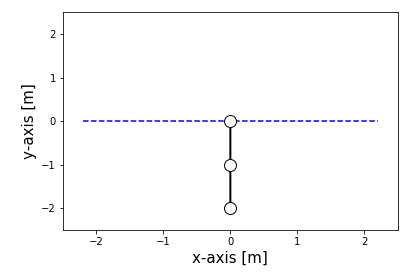
\includegraphics[width=1\textwidth]{img/2finitialpos.png} 
				\captionof{figure}{Task Space Control: Initial Position}
				\label{fig:2f3}            
			\end{minipage}%
			\begin{minipage}{.5\textwidth}
             Comparing the actual end position with the desired end position(-0.35,1.5) in task space:\\
             \begin{tabular}{ l l l }
             	method & endx & endy \\
             	JacTrans & -0.366 & 1.476 \\
             	JacPseudo &  0.137 & 1.1264 \\
             	JacDPseudo & -0.326 & 1.512 \\
             	JacNullSpace[0,pi] & -0.3247 & 1.512 \\
             	JacNullSpace[0,-pi] & -0.2985 & 1.4905 \\
             \end{tabular}
			\end{minipage}


			\noindent\begin{minipage}{.5\textwidth}
				\centering
				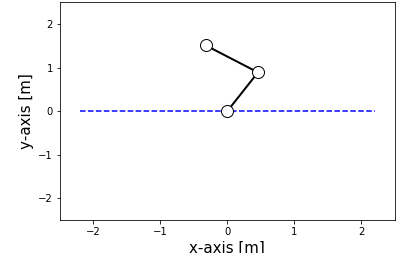
\includegraphics[width=1\textwidth]{img/2f0pi.png} 
				\captionof{figure}{Task Space Control Jac Null Space with resting pose [0,pi]}
				\label{fig:2f1}            
			\end{minipage}%
			\begin{minipage}{.5\textwidth}
				\centering
				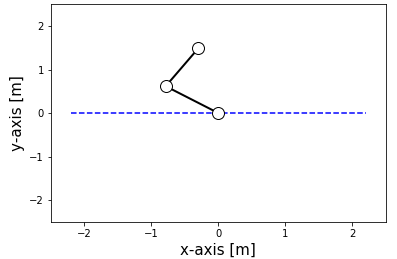
\includegraphics[width=1\textwidth]{img/2f0-pi.png} 
				\captionof{figure}{Task Space Control Jac Null Space with resting pose [0,-pi]}
				\label{fig:2f2}                 
			\end{minipage}

Using the JacDPseudo method the desired position is almost reached. However using the JacNullSpace method the desired position is approximated in two different ways one from the "left" (see \ref{fig:2f1}) and one from the right (see \ref{fig:2f2})

My\_taskspace.py:\\
\pythonexternal{src/mytaskspace.py}
	
	
	\end{answer}
		
	\end{question}
	
\end{questions}

